\documentclass{article}
\setlength{\topmargin}{-1in}
\setlength{\oddsidemargin}{0in}
\setlength{\textwidth}{6.25in}
\setlength{\textheight}{10in}
\usepackage{bm}
\usepackage{amsmath}
\usepackage{graphicx}
\usepackage{subfigure}

\begin{document}
\title{Confidence-Weighted Sparse Online Learning}
\author{Yue Wu}
\maketitle

\section{Introduction}
The main idea of Confidence-Weighted algorithms is to assume a Guassian distribution 
of the linear classifier $\bm{\omega}\sim N(\bm{\mu},\Sigma)$. Each update
tries to stay close to the previous distribution and ensure the
probability of the current precision for $\bm{x}_i$ is larger than
$\eta$.
\begin{equation}
  \begin{aligned}
    Pr[y_i(\bm{\mu}\cdot \bm{x}_i) \geq 0]  \geq \eta \quad or \quad
    y_i(\bm{\mu}\cdot \bm{x}_i)  \geq  \phi\sqrt{\bm{x}_i^T\Sigma\bm{x}_i}
  \end{aligned}
  \label{equ:01}
\end{equation}

\section{Problem Formulation}
In Sparse online learning, we set the weight vector equal to the average
$\bm{\omega} = \bm{\mu}$. Each iteration step is a minimization problem as follows:
\begin{equation}
    \bm{\mu}_{t} = \arg\min_{\bm{\mu}}{f(\bm{\mu}) + \tilde{\lambda} r(\bm{\mu})}
    \label{equ:02}
\end{equation}
where $f(\bm{\mu})$ is often the loss function. In this paper, we follow the
setting of AROW and use the squared hinge loss:
\begin{equation}
    f(\bm{\mu}) = \max(0, 1 - y_t (\bm{\mu_t}\cdot \bm{x}_t))^2
    \label{equ:03}
\end{equation}

To the regularization term, previous learning algorithms treat all the
coordinates the same by adding an regularization term
$\lambda|\omega|$. We extend the confidence to apply different
regularization intensities to different coordinates. A high variance value
corresponds a low confidence.  Accordingly, we apply a strong shrinkage to
less confident coordinates and weak shrinkage to confident ones.

\subsection{Smooth Regularization}
Smooth regularization is the \textit{L1} norm. We call it smooth 
sparse regularization, as it shrink the weight values by some amount once a
iteration.
\begin{equation}
    r(\bm{\mu})  = |\Sigma\bm{\mu}|
    \label{equ:04}
\end{equation}

\subsection{Aggressive Regularization}
Aggressive regularization is a strict condition on the number of non-zero
coordinates, as Equ \ref{equ:05} shows. This setting is useful in problems like feature selection.
\begin{equation}
    r(\bm{\mu}) = \left\{
        \begin{aligned}
            0, \quad & |\Sigma\bm{\mu}|_0 \leq B \\
            \infty, \quad & |\Sigma\bm{\mu}|_0 > B
        \end{aligned}
        \right.
    \label{equ:05}
\end{equation}

\section{Solution}
Common approaches such as subgradient methods to Equ. \ref{equ:01} will rarely
lead to non-differential points of $f(\bm{\omega})$ or $r(\bm{\omega})$. While
these non-differential points are the true minima in cases like \textit{L1}
regularization. Instead, we adopt a \emph{forward-backward splitting} approach
to alleviate the problems of non-differentiability.

In the first step, we adopt AROW on $f(\mu)$ to obtain one step iteration. The
iteration is as Equ \ref{equ:06} shows.
\begin{equation}
    \begin{aligned}
        \bm{\mu}_{t - \frac{1}{2}} = \bm{\mu}_{t-1} + \alpha_t\Sigma_{t-1}y_t\bm{x}_{t} \quad & \quad
        \Sigma_t = \Sigma_{t-1} - \beta_t\Sigma_{t-1}\bm{x}_t\bm{x}_t^T\Sigma_{t-1}\\
        \beta_t = \frac{1}{\bm{x}_t^T\Sigma_{t-1}\bm{x}_t + r} \quad & \quad
        \alpha_t = \max(0, 1 - y_t
        \bm{x}_t^T\bm{\mu}_{t-1})\beta_t
    \end{aligned}
    \label{equ:06}
\end{equation}

We re-write the above iteration to be second order sub-gradient update as Equ.
\ref{equ:07}.
\begin{equation}
    \begin{aligned}
        \bm{\mu}_{t - \frac{1}{2}} &= \bm{\mu}_{t-1} -
        \frac{\beta_t}{2}\Sigma_{t-1}g_t^f\\
        g_t^f &= \partial{f(\bm{\mu})} 
    \end{aligned}
    \label{equ:07}
\end{equation}

In the above update equation, $\frac{\beta_t}{2}$ is the common learning rate.
$\Sigma_{t-1}$ is the matrix to apply different learning rates to different
coordinates.

The second step is a projection step with the smooth regularization penalty.
\begin{equation}
    \begin{aligned}
        \tilde{\lambda} &= \frac{\beta_t}{2} \lambda \\
        \bm{\mu}_{t} &= \arg\min_{\mu}{\frac{1}{2}\|\bm{\mu} -
        \mu_{t-\frac{1}{2}}\|^2
        + \frac{\beta_t}{2}\lambda|\Sigma_{t-1}\mu|}
    \end{aligned}
    \label{equ:08}
\end{equation}


The final updating rule goes to:
\begin{equation}
    \mu_{t,j} = sign(\mu_{t-1,j} -
    \frac{\beta_t}{2}\Sigma_{t-1,jj}g_{t-1,j}^f)
    [|\mu_{t-1,j} - \frac{\beta_t}{2}\Sigma_{t-1,jj}g_{t-1,j}^f| -
    \frac{\beta_t}{2}\lambda\Sigma_{jj}]
    \label{equ:09}
\end{equation}

\section{Experimental results}
\subsection{Experiment on real datasets}

\begin{table}[!ht]
% increase table row spacing, adjust to taste
\renewcommand{\arraystretch}{1.3}
 %\extrarowheight 
\caption{Real Datasets}
\label{tbl:01}
\centering
\begin{tabular}{|c|c|c|c|c|c|}
\hline
DataSet& Feat Dim & Train Data No. & Test Data No. & Feat No. & sparsity\\
\hline
MNIST67 & 780 & 12183 & 1987 & 1,751,945 & 0\\
\hline
news & 732209 & 9960 & 9994 & 5,513,533 & 0\\
\hline
rcv1& 47,152  & 781,265 & 23,149 &59,155,144 & 0\\
\hline
url\_combined & 3,231,961 & 2,000,000 & 396,130 &231,259,917 & 0\\
\hline
webspam& 16,609,143 &300,000 & 50,000 &1, 118,443,083 & 0\\
\hline
\end{tabular}
\end{table}

\subsection{test error rate vs sparsity}
\subsubsection{TG-based algorithms}
\begin{figure}[!h]
\centering
\subfigure[MNIST]{
    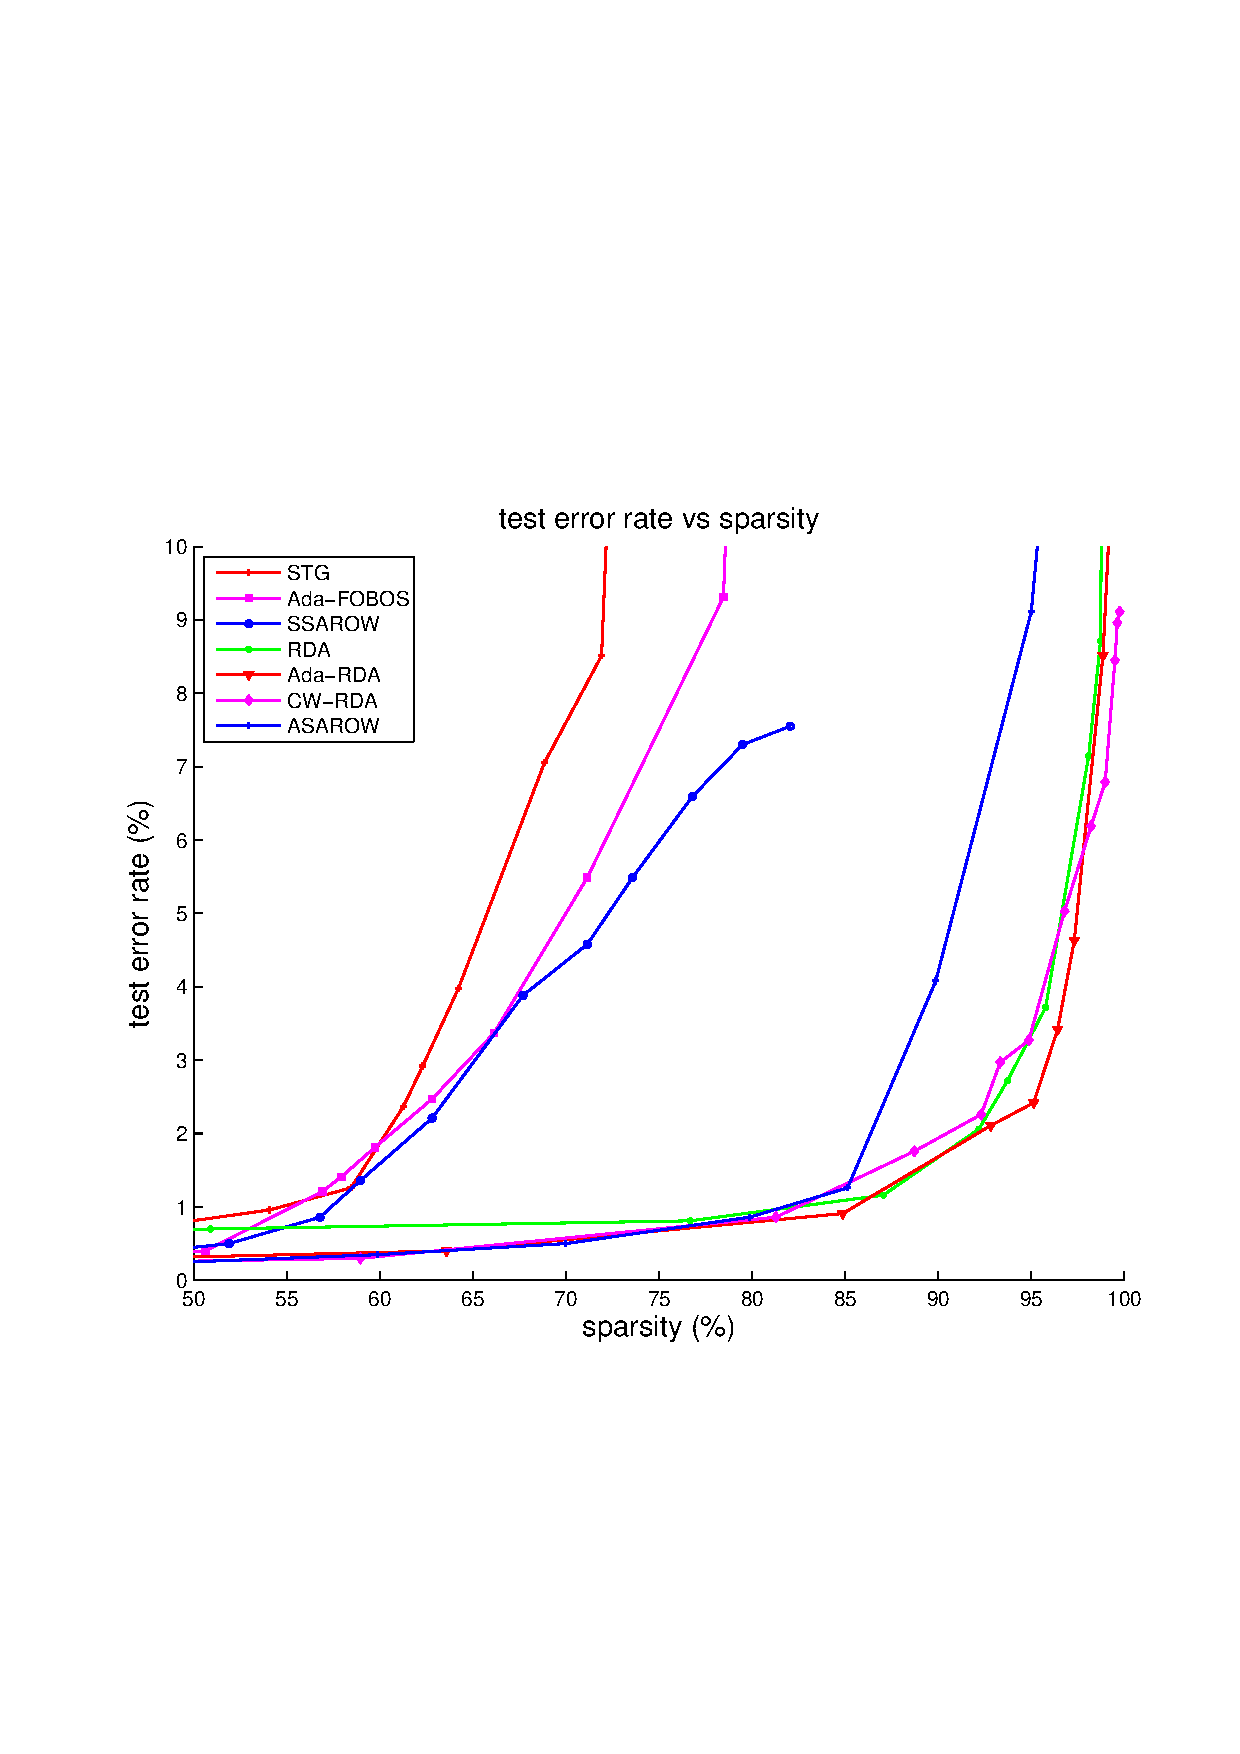
\includegraphics[width=0.33\textwidth]{./figs/MNIST67_test.pdf}}
\subfigure[news]{
    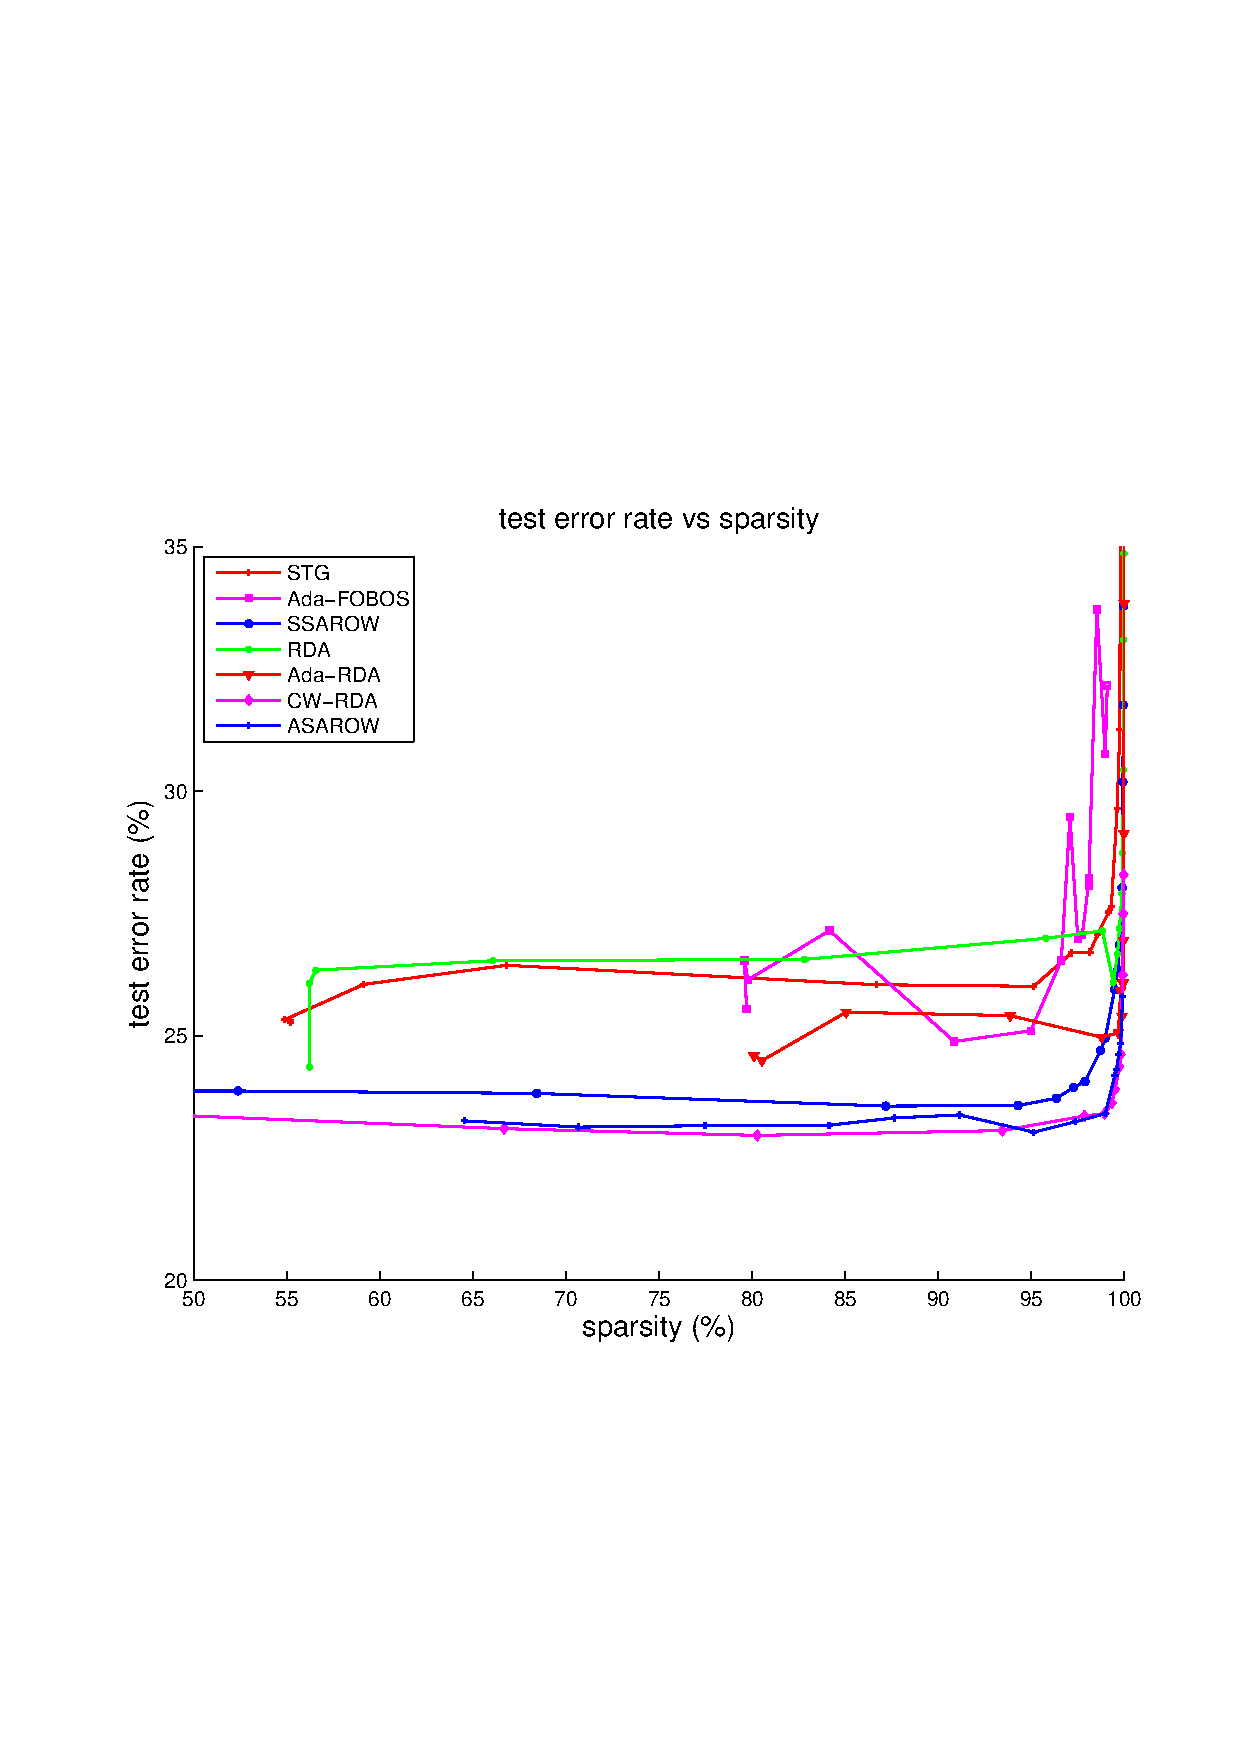
\includegraphics[width=0.33\textwidth]{./figs/news_test.pdf}}
\subfigure[rcv1]{
    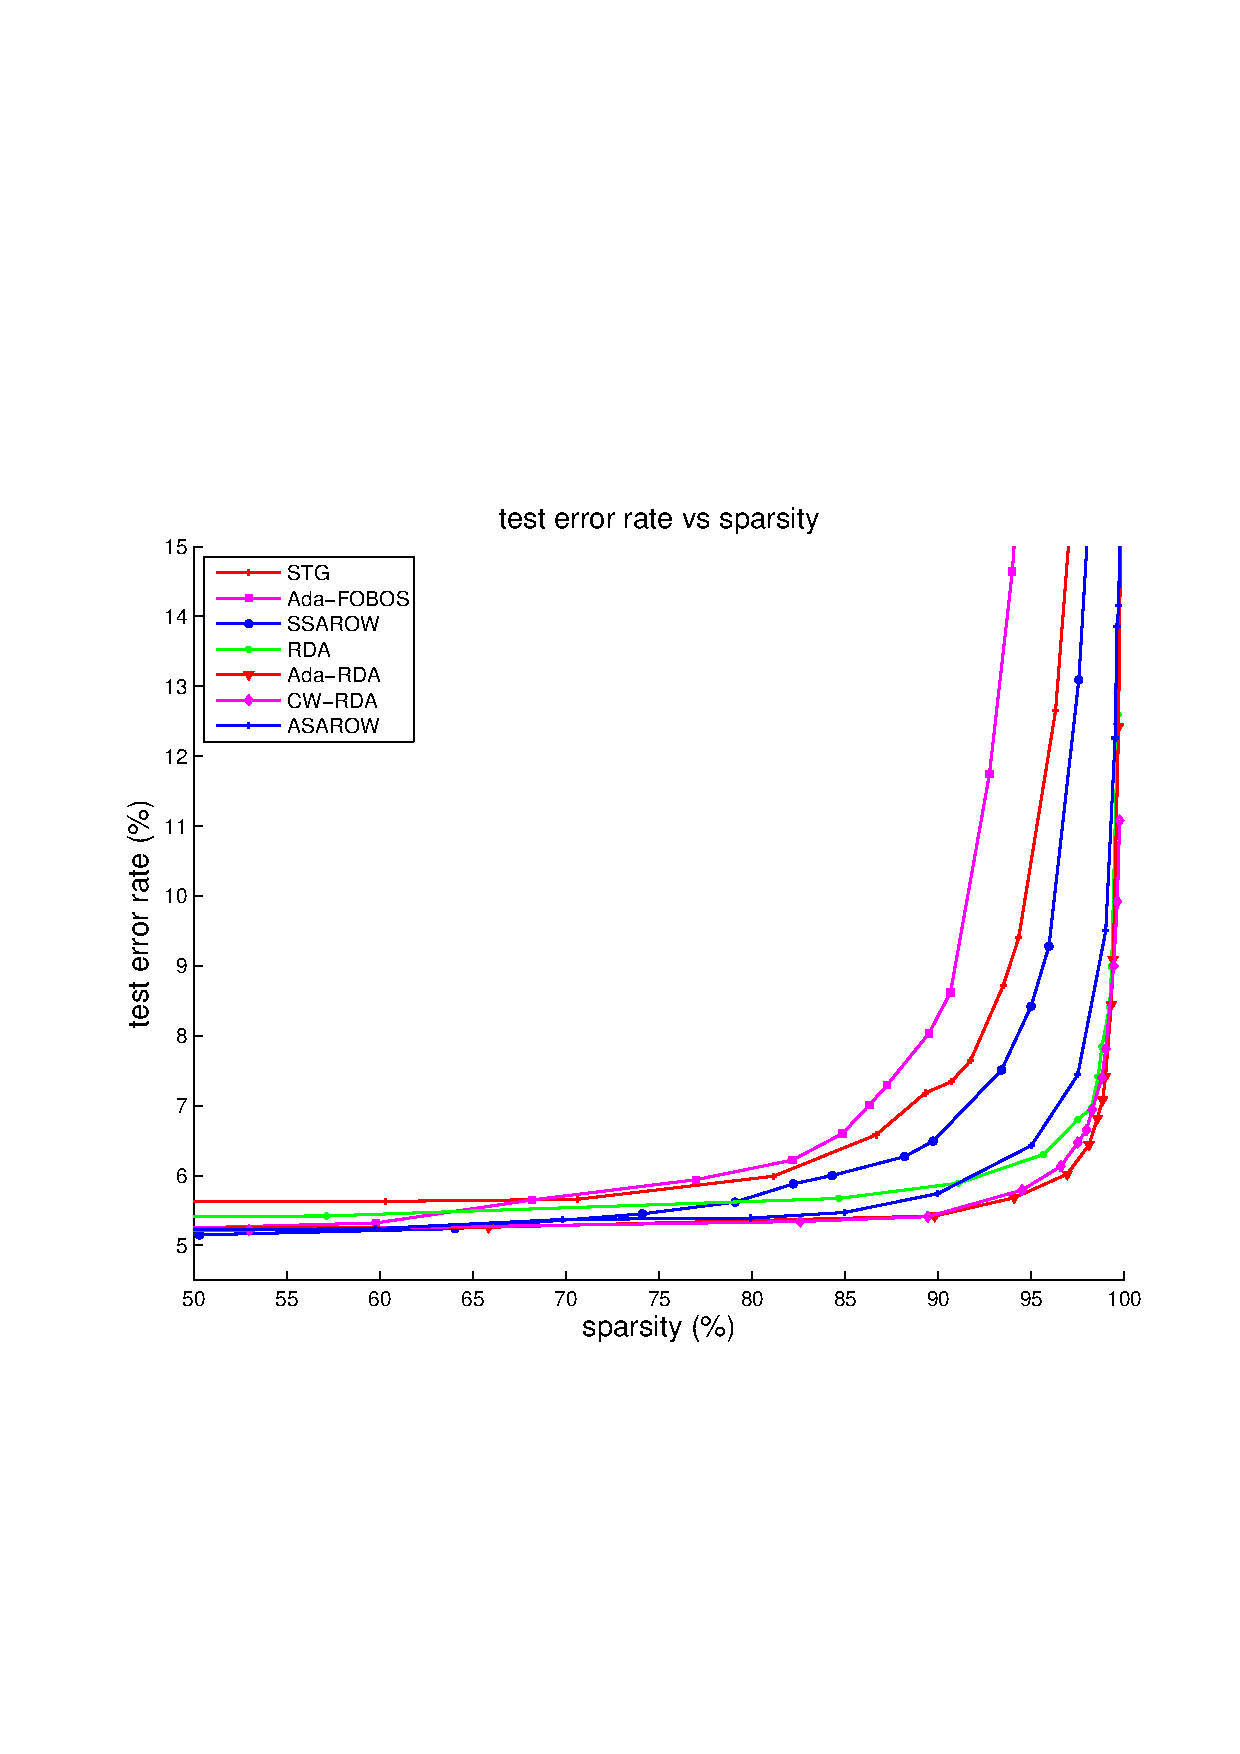
\includegraphics[width=0.3\textwidth]{./figs/rcv1_test.pdf}}
\subfigure[url]{
    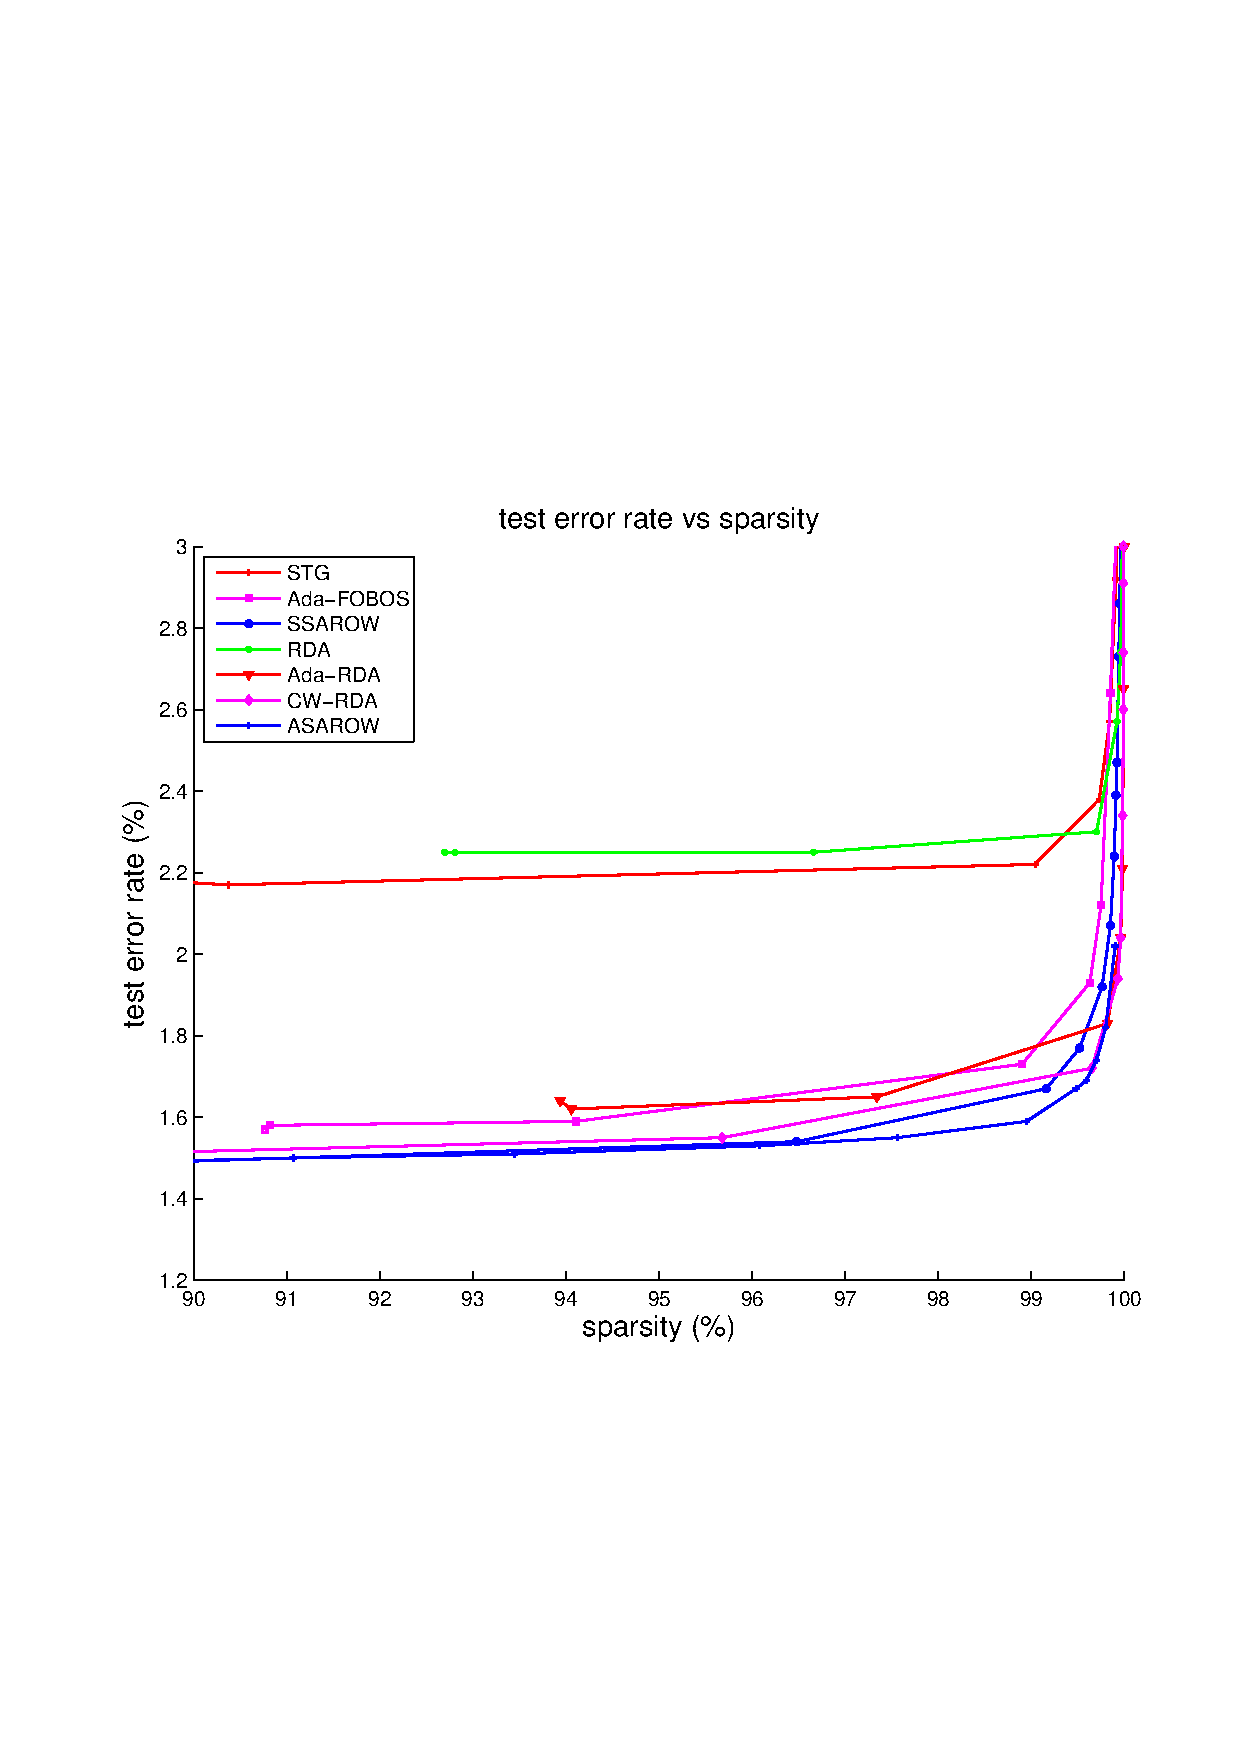
\includegraphics[width=0.3\textwidth]{./figs/url_test.pdf}}
\subfigure[webspam]{
    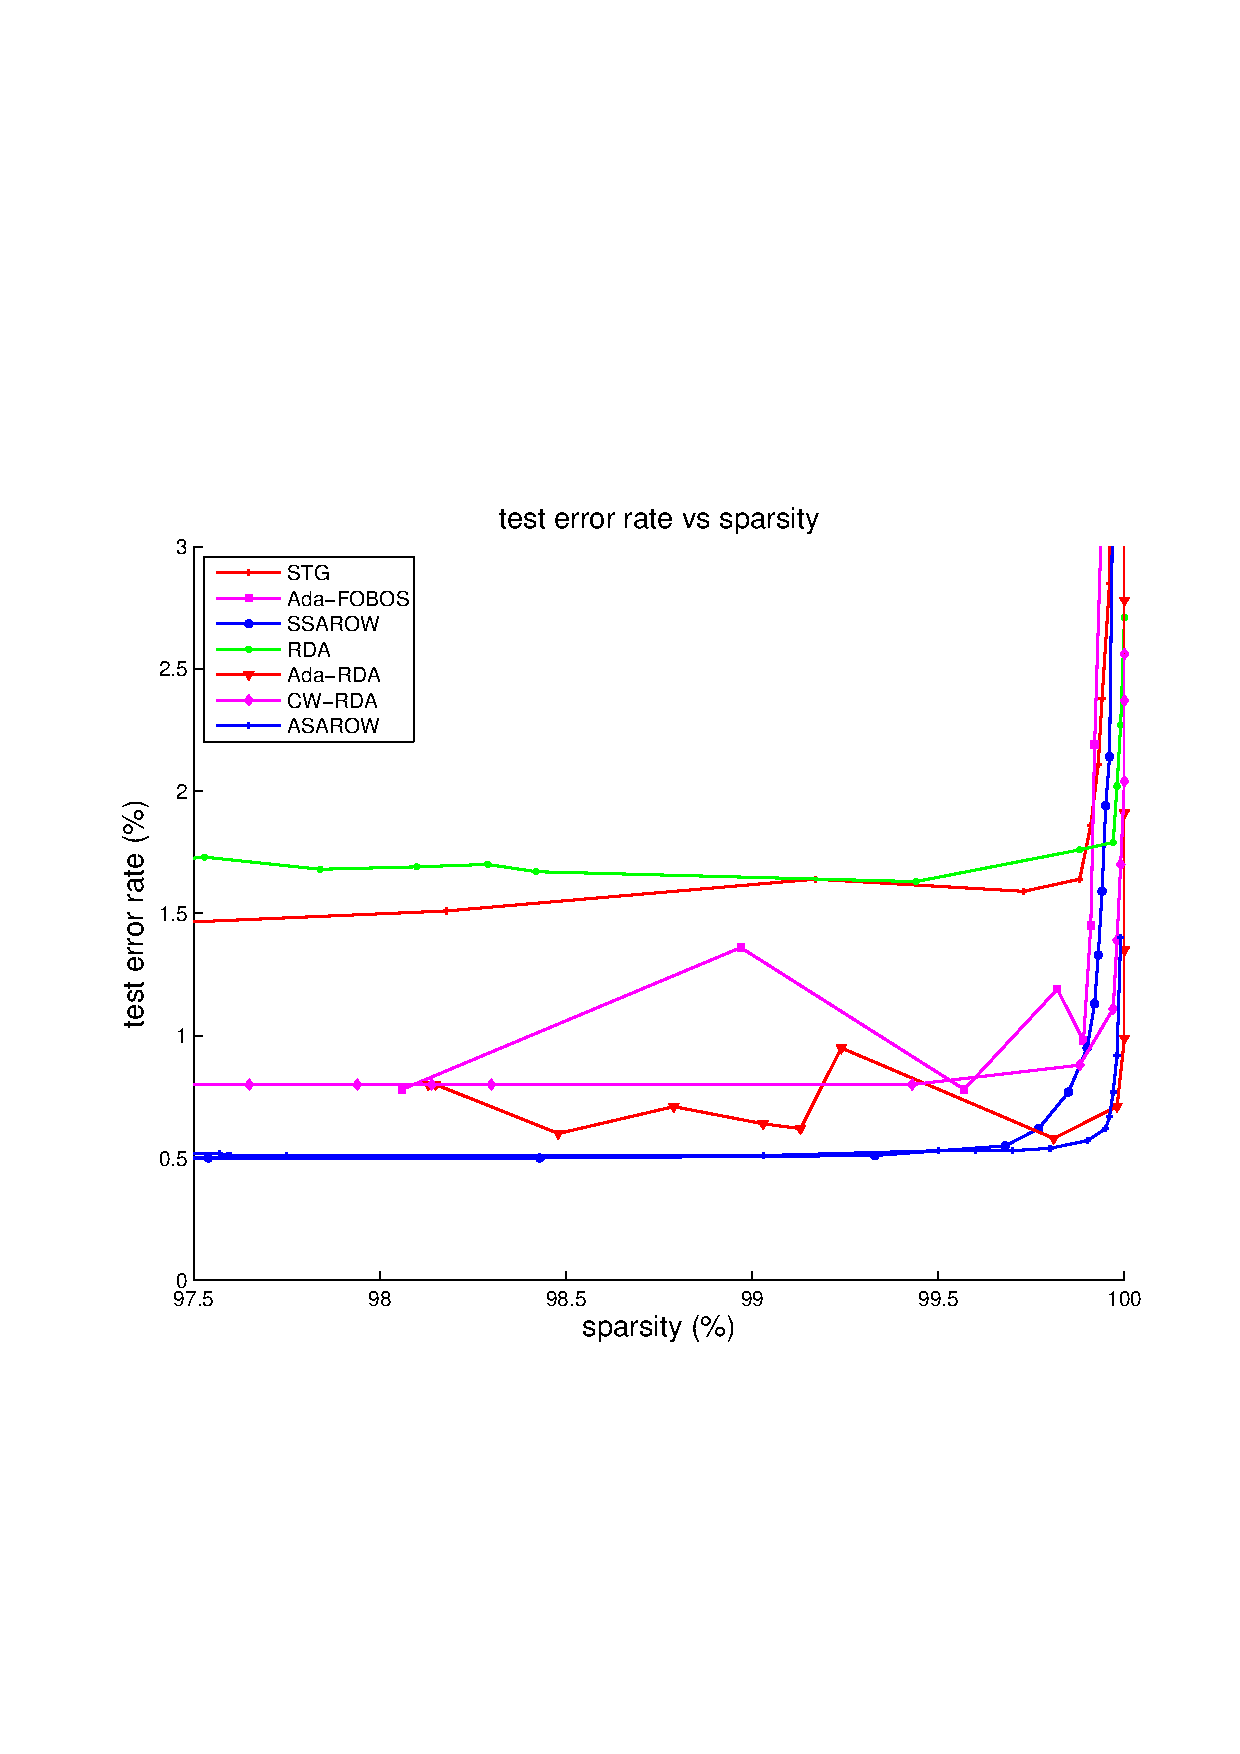
\includegraphics[width=0.33\textwidth]{./figs/webspam_trigram_test.pdf}}
\label{fig:00}
\end{figure}

\subsubsection{DA-based algorithms}
\begin{figure}[!h]
\centering
\subfigure[MNIST]{
    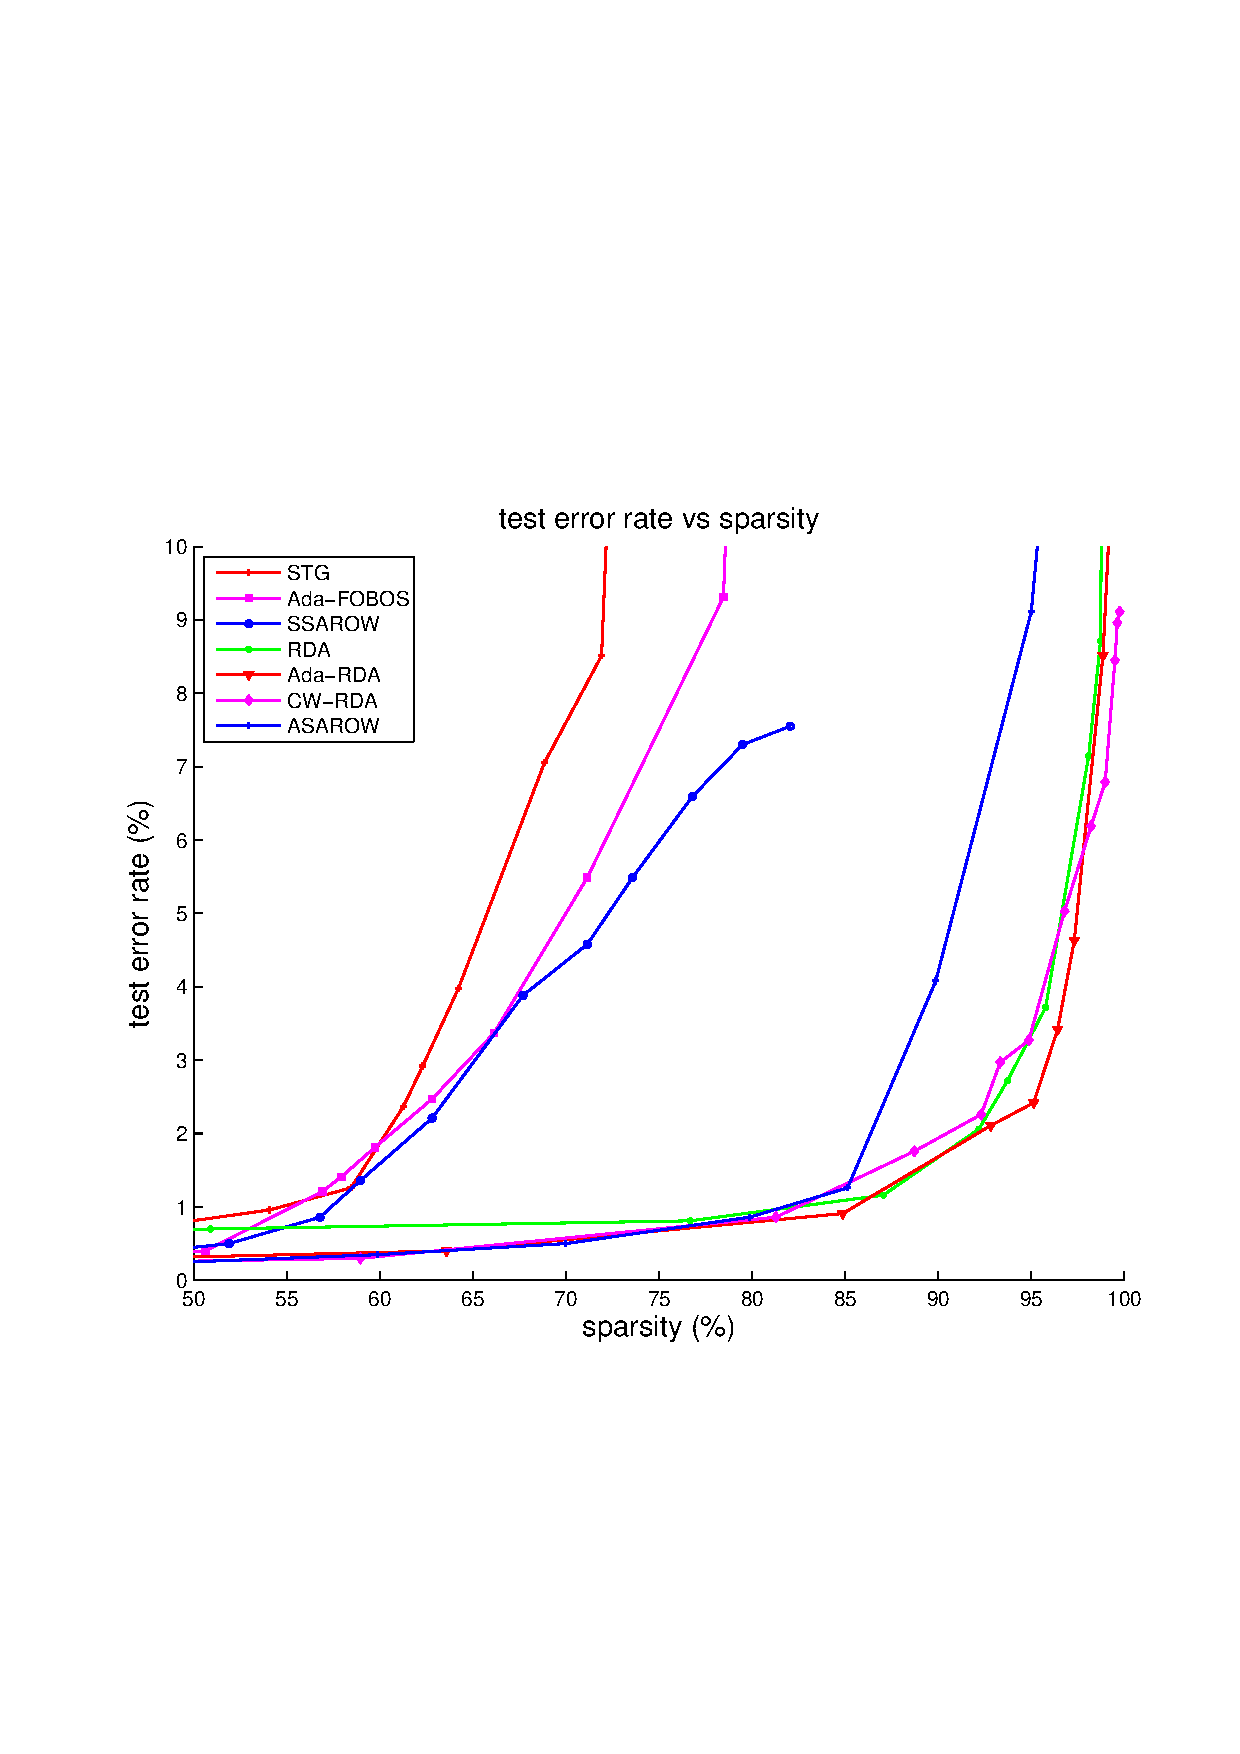
\includegraphics[width=0.33\textwidth]{./figs/MNIST67_test.pdf}}
\subfigure[news]{
    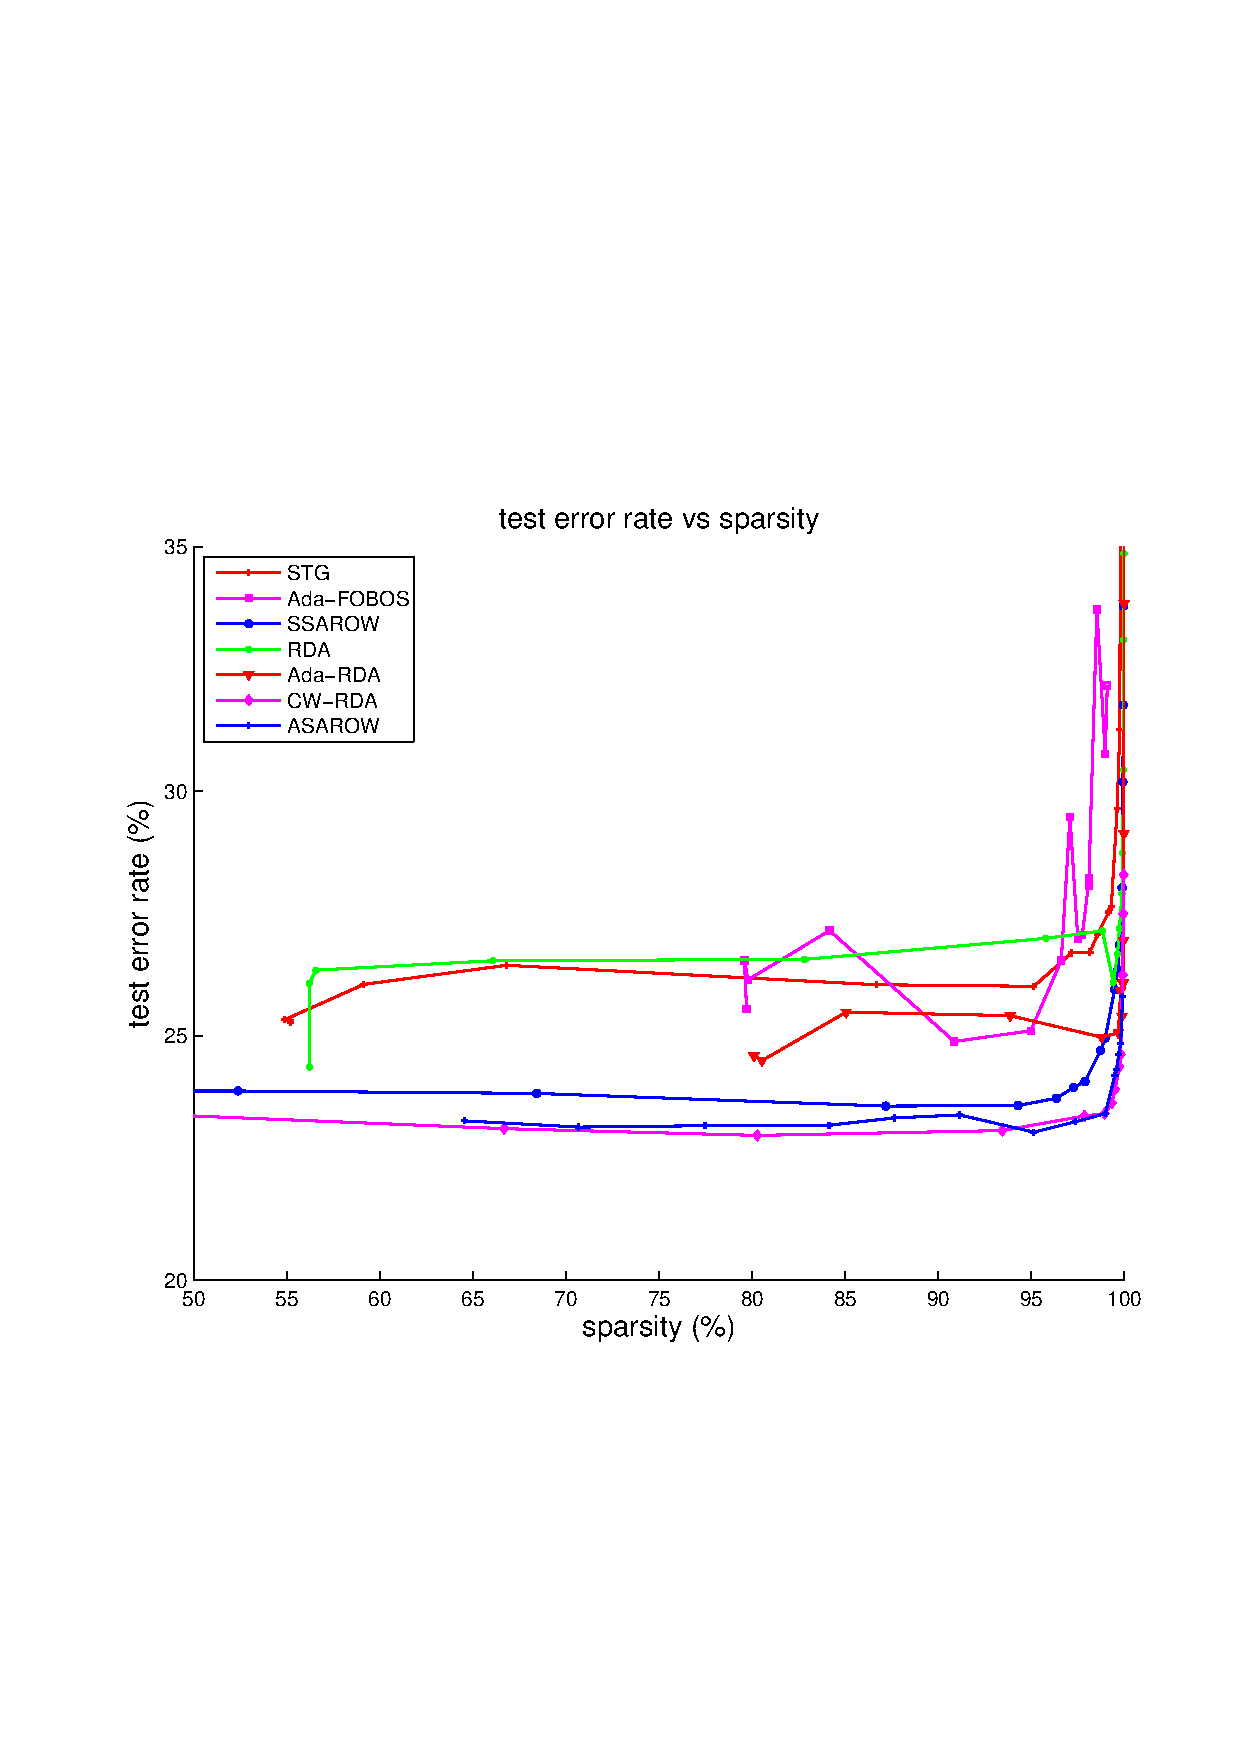
\includegraphics[width=0.33\textwidth]{./figs/news_test.pdf}}
\subfigure[rcv1]{
    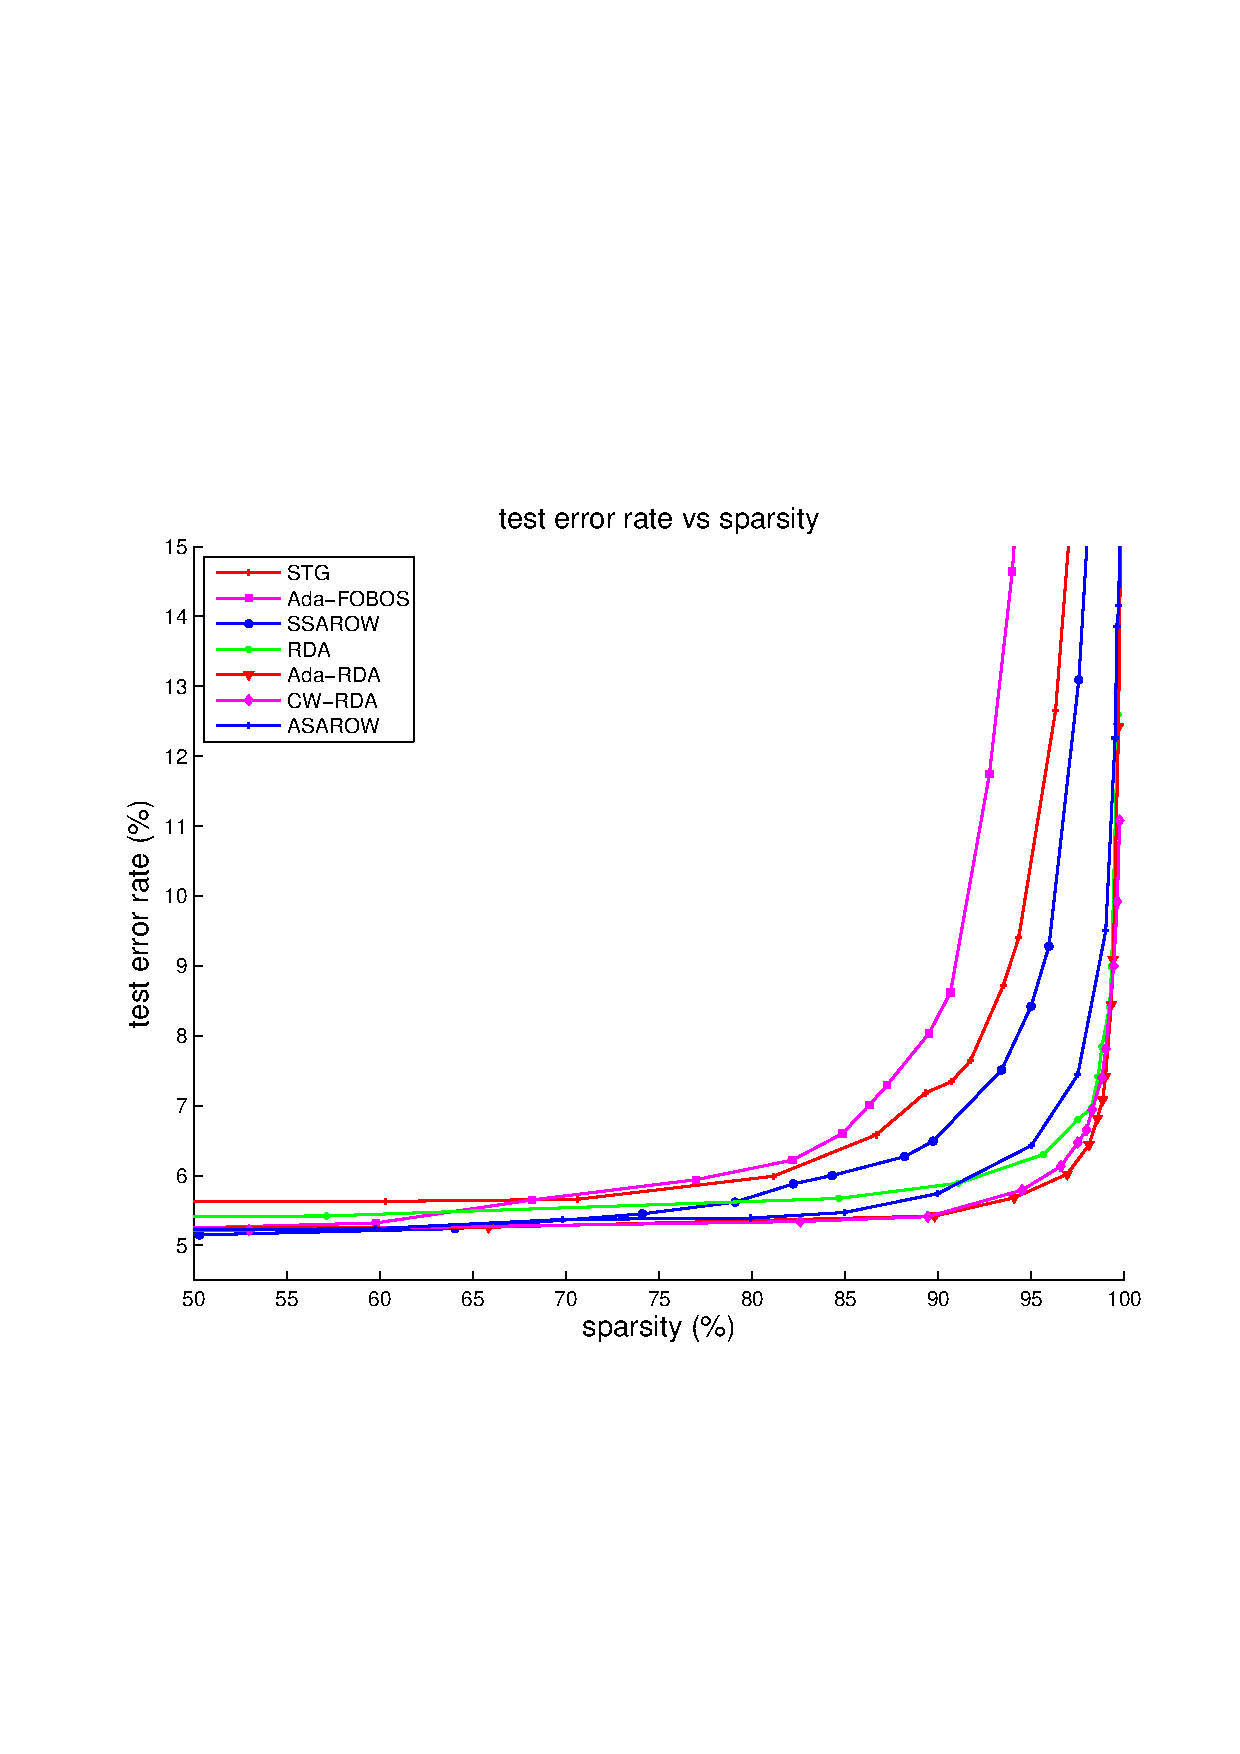
\includegraphics[width=0.3\textwidth]{./figs/rcv1_test.pdf}}
\subfigure[url]{
    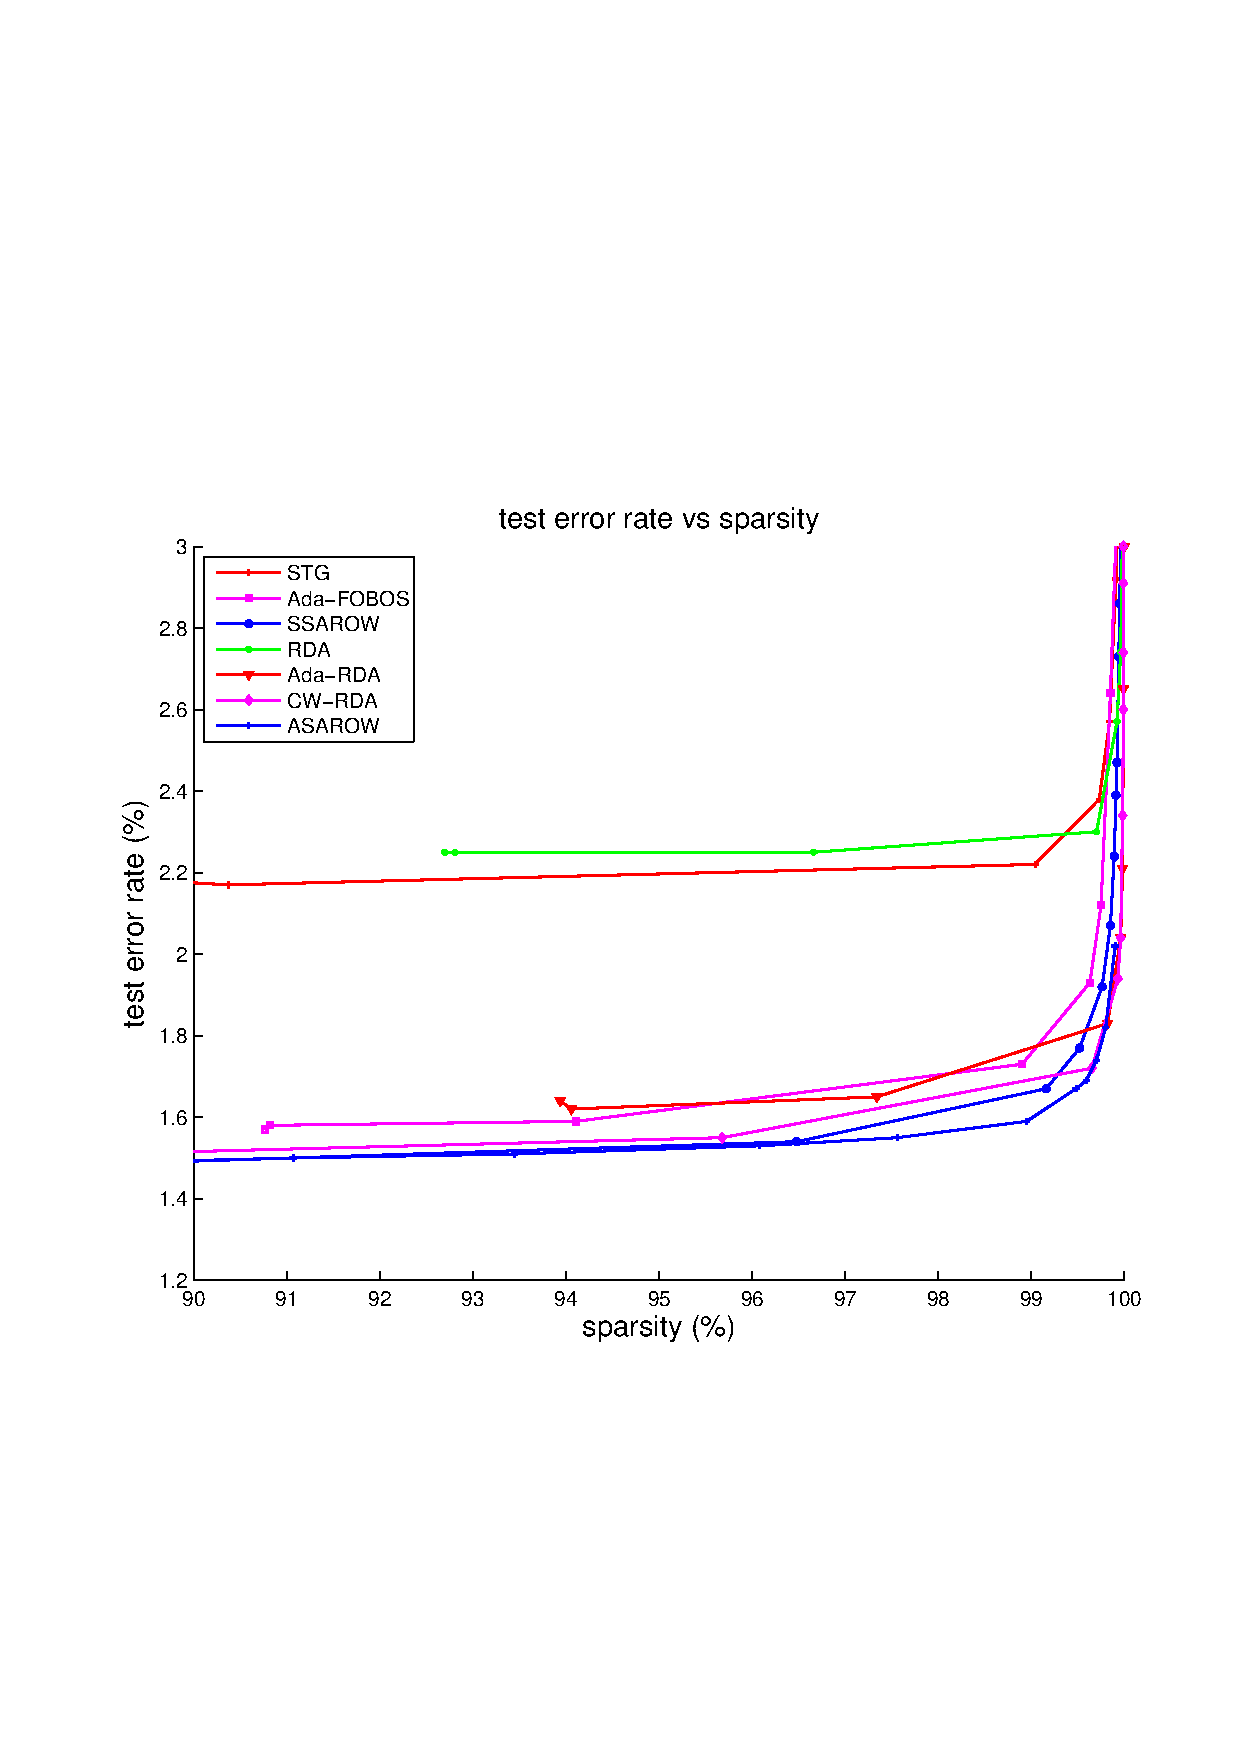
\includegraphics[width=0.3\textwidth]{./figs/url_test.pdf}}
\subfigure[webspam]{
    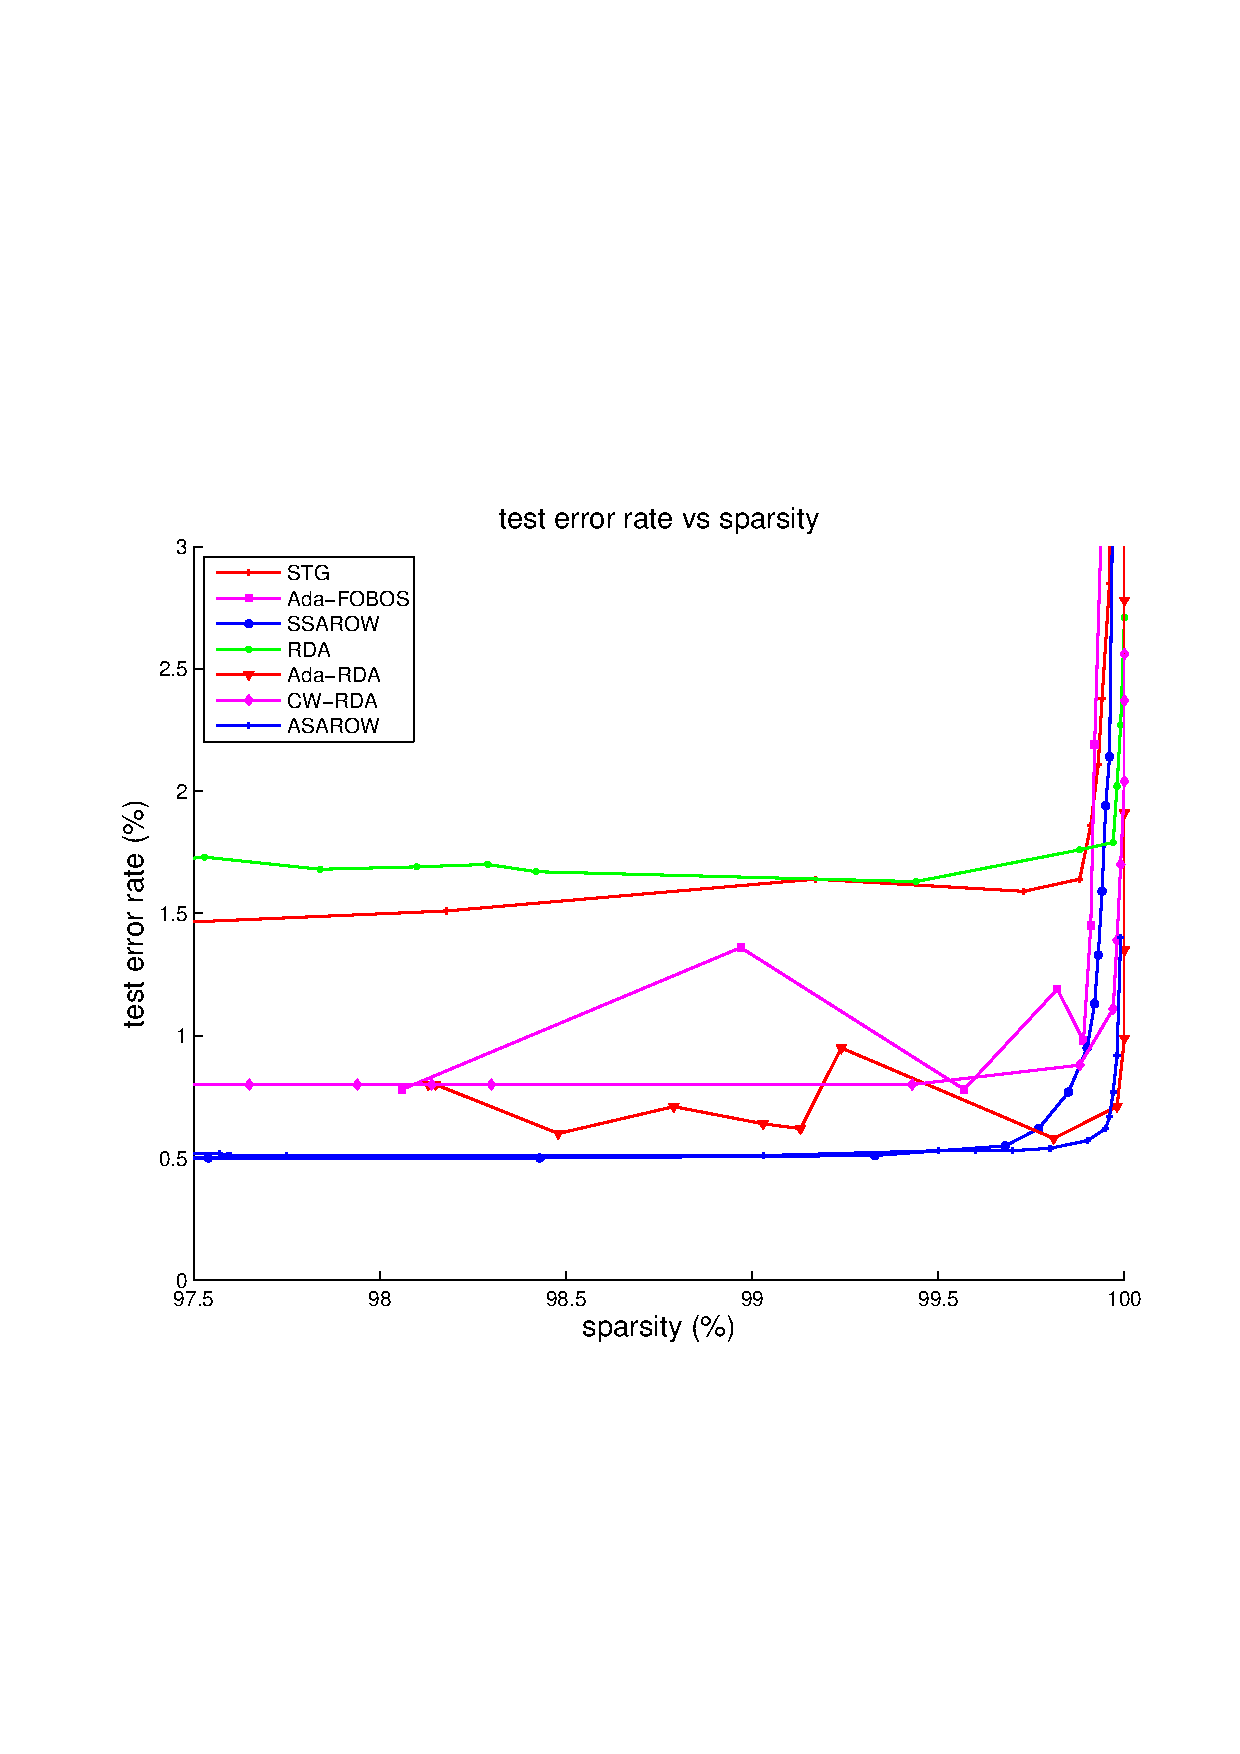
\includegraphics[width=0.33\textwidth]{./figs/webspam_trigram_test.pdf}}
\label{fig:01}
\end{figure}

\section{Reference}

\end{document}
